\subsection {Approximation of High order Polynomial solving 1D Poisson Equation}

In this section we construct a polynomial $P_n$ of order $n$
defined on $[0,1]$, which satisfies the following.
\begin{eqnarray*}
 P_n(0) = 0, &P_n(1) = 1 \\
 \frac{d^k}{dx^k}P_n(0) = 0, &\frac{d^k}{dx^k}P_n(1) = 0
\end{eqnarray*}
for all $k = 1, \cdots, n-2$. \\
Then for each $n$, we obtain a polynomial $P_n$ by solving a
system of linear equations having unique solution which determines
the set of coefficients of $P_n$. We will apply the spectral
polynomial solver to approximate the second derivative $Q_{n-2}$
of $P_n$.

\subsubsection{Polynomial Representation of Approximation using Legendre Basis}




Figure \ref{sol1} is showing some samples of solution of
order($n$) $9$.

\begin{problem}
\label{problem2}Consider the following differential equation for
$u(x)$ such that
\begin{equation*}
    \frac{d^2}{dx^2} u(x) = Q_{n-2},
\end{equation*}
for all $x$ in $[0, 1]$. Then the problem is to find approximation
$p(x)$ of $u(x)$ using spectral polynomial method.
\end{problem}

\noindent



\subsubsection{Existence of Approximate Solution}

The Figure \ref{crvconvf1} and \ref{crvconvf2} are showing the
result of spectral polynomial method approximating the solution of
Problem \ref{problem2}. The maximum error value in Table
 \ref{crvconv1t} is showing the approximation is within numerically
exact solution tolerance.

\clearpage
%----------------------------------------------------------------------

\subsubsection{Convergence of Solution in H-test}


\begin{itemize}

\item Dirichlet-Dirichlet Case
\begin{figure}[h]
\begin{center}
\epsfig{file = figs_dd/ScrvHconv.eps, %
        height = 9cm}
\caption{\label{ScrvHconv}Graph showing change of errors by the
increase of the number of elements: Dirichlet-Dirichlet}
\end{center}
\end{figure}

\begin{table}[h]
\centering \caption{\label{ScrvHconvt} Specification of
                              Figure\ref{ScrvHconv} and their errors}
\begin{tabular}{|c|c|c|} \hline
Polynomial order&Error&Slope   \\ \hline \hline
    3&$7.5505e-011$ &$3.9909$ \\ \hline
    4&$3.1679e-013$ &$4.7538$ \\ \hline
    5&$9.4591e-014$ &$5.5248$ \\ \hline
\end{tabular}
\end{table}


\item Dirichlet-Neumann Case

\begin{figure}[h]
\begin{center}
\epsfig{file = figs_dn/ScrvHconv.eps, %
        height = 9cm}
\caption{\label{ScrvHconv}Graph showing change of errors by the
increase of the number of elements: Dirichlet-Neumann}
\end{center}
\end{figure}

\begin{table}[h]
\centering \caption{\label{ScrvHconvt} Specification of
                              Figure\ref{ScrvHconv} and their errors}
\begin{tabular}{|c|c|c|} \hline
Polynomial order&Error&Slope   \\ \hline \hline
    3&$7.5530e-011$ &$3.9908$ \\ \hline
    4&$4.5619e-013$ &$4.6486$ \\ \hline
    5&$4.1855e-013$ &$5.7218$ \\ \hline
\end{tabular}

\end{table}


\end{itemize}

%\clearpage
%----------------------------------------------------------------------

\subsubsection{Test of Convergence of Solution in Variable Ordered
Elements}



\begin{itemize}

\item Dirichlet-Dirichlet Case
\begin{figure}[h]
\begin{center}
\epsfig{file = figs_dd/ScrvPconv.eps, %
        height = 9cm}
\caption{\label{ScrvPconv}Graph showing change of errors by the
increase of the number of elements: Dirichlet-Dirichlet}
\end{center}
\end{figure}

\begin{table}[h]
\centering \caption{\label{ScrvPconvt} Specification of
                              Figure\ref{ScrvPconv} and their errors}
\begin{tabular}{|c|c|} \hline
Number of Elements&Error   \\ \hline \hline
    5&$5.5067e-014$  \\ \hline
    10&$7.9936e-014$  \\ \hline
\end{tabular}
\end{table}


\item Dirichlet-Neumann Case

\begin{figure}[h]
\begin{center}
\epsfig{file = figs_dn/ScrvPconv.eps, %
        height = 9cm}
\caption{\label{ScrvPconv}Graph showing change of errors by the
increase of the number of elements: Dirichlet-Neumann}
\end{center}
\end{figure}

\begin{table}[h]
\centering \caption{\label{ScrvPconvt} Specification of
                              Figure\ref{ScrvPconv} and their errors}
\begin{tabular}{|c|c|} \hline
Number of Elements&Error   \\ \hline \hline
    5&$3.0431e-013$  \\ \hline
    10&$3.1186e-013$ \\ \hline
\end{tabular}

\end{table}


\end{itemize}
